\section{Installation}\label{installation}

StarRiver Server has two modules: database system and StarRiver
communication application.

\subsection{Prerequisites}\label{prerequisites}

StarRiver Server relies on .Net Framework 4.0. Please install the
framework at the very beginning to prevent possible issues during
installation of other modules.

The installer can be found at
\href{https://www.microsoft.com/en-US/download/details.aspx?id=17718}{Microsoft's
webpage}. A copy is provided in the StarRiver installation disk.

\subsection{Database Installation}\label{database-installation}

StarRiver works with MySQL or its compatible replacements such as
MariaDB. The following guide is based on MySQL Server 5.6 as an example.

First, download the installer from the
\href{http://dev.mysql.com/downloads/mysql/}{MySQL website}. The MySQL
Installer packaged for Windows platform is recommended.
\href{http://dev.mysql.com/downloads/windows/installer/5.6.html}{MySQL
Installer 5.6.19} is adopted here.

Here are the installation steps.

\begin{enumerate}
\def\labelenumi{\arabic{enumi}.}
\itemsep1pt\parskip0pt\parsep0pt
\item
  The installer shows a welcome page initially. Select ``Install MySQL
  Products''. 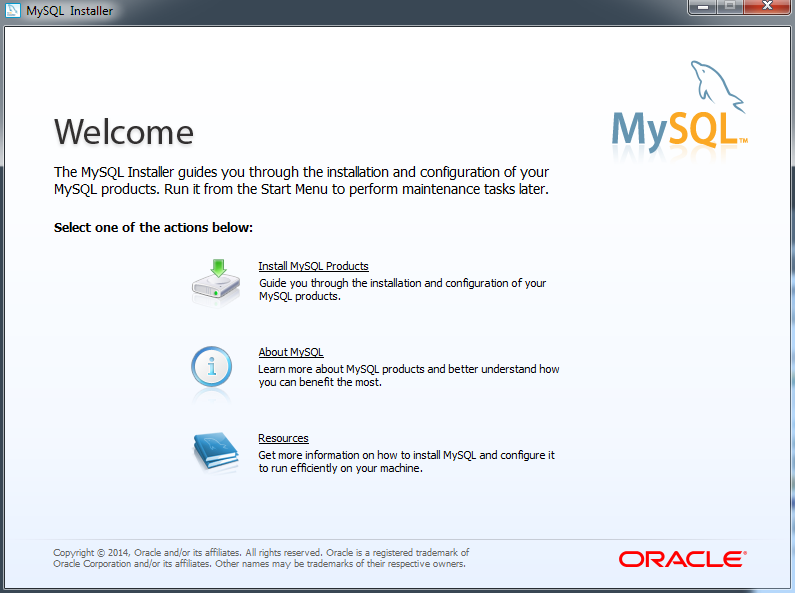
\includegraphics{img/mysql_1.png}
\item
  Now the installer checks for updates. If there is no Internet
  connection, tick ``Skip the check for updates'' and continue.
  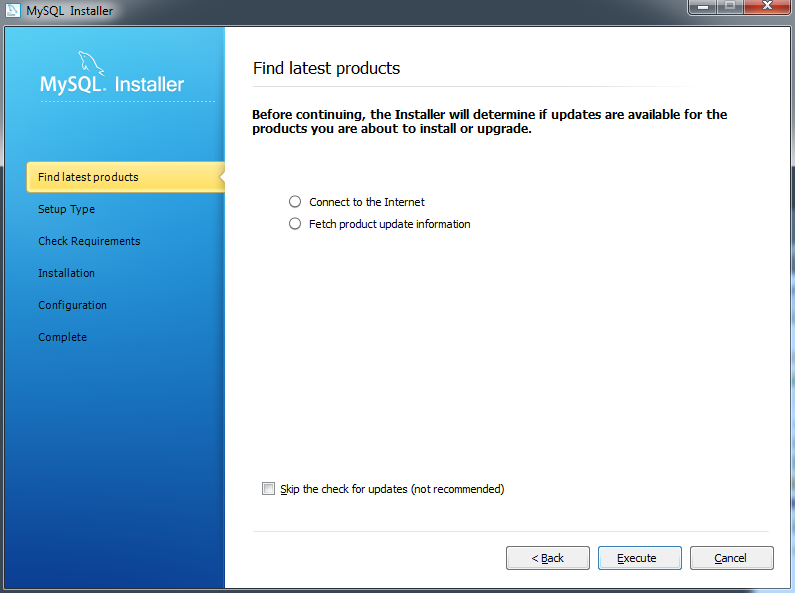
\includegraphics{img/mysql_2.png}
\item
  Select ``Server only'' as the setup type and specify the data path.
  Here we use \texttt{C:\textbackslash{}MySQL\_Data} as an example.
  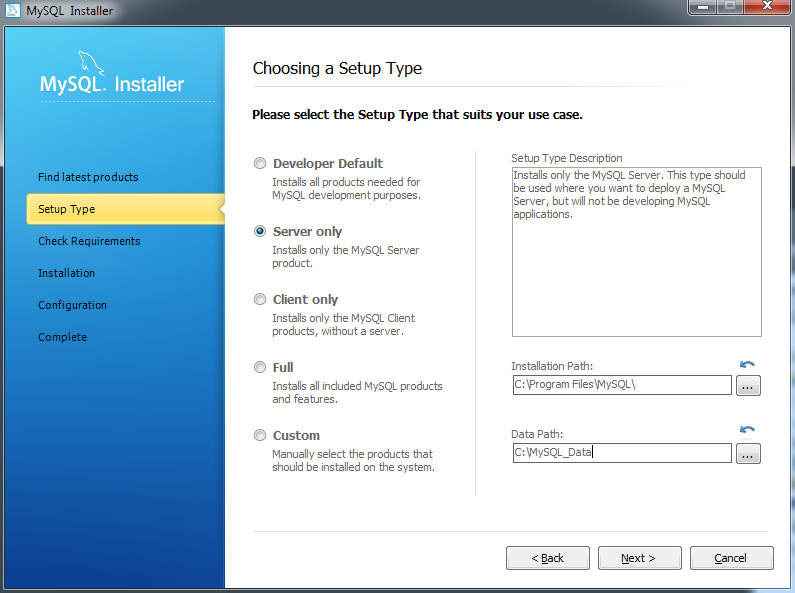
\includegraphics{img/mysql_3.png}
\item
  The installer will check for addition requirements to be installed.
  Let it finish. 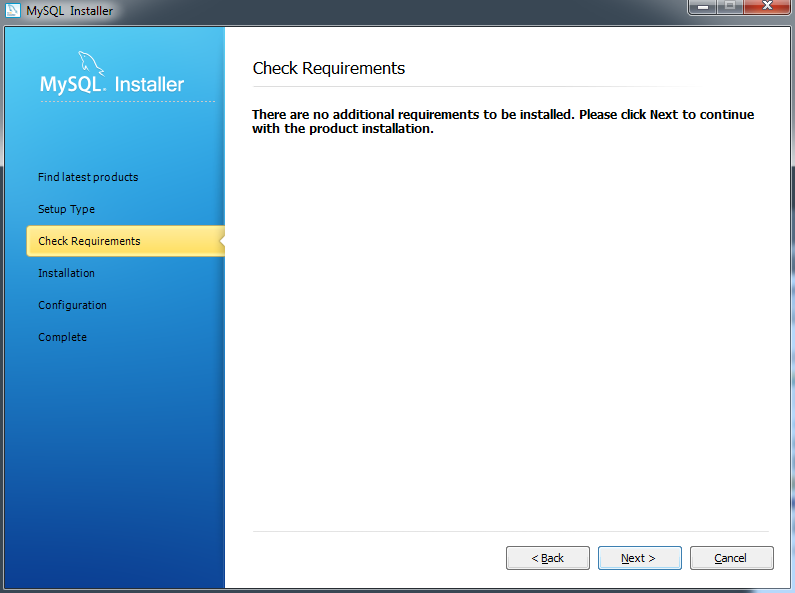
\includegraphics{img/mysql_4.png}
\item
  Click ``Execute'' to install MySQL Server.
  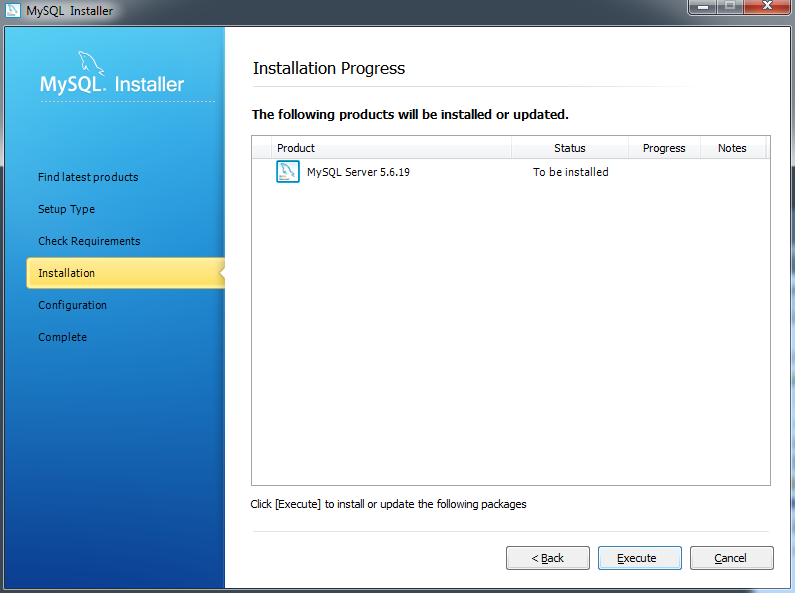
\includegraphics{img/mysql_5.png}
\item
  Installation finishes. Click ``Next'' to start configuration.
  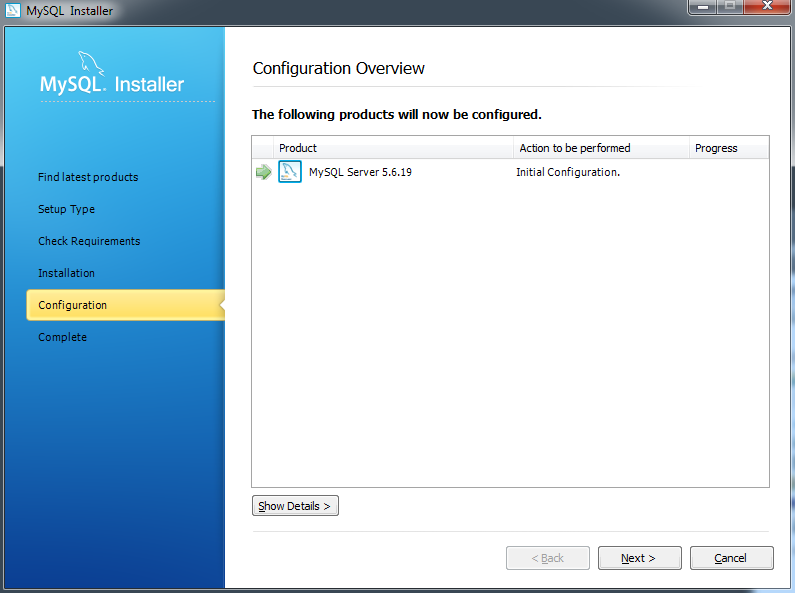
\includegraphics{img/mysql_6.png}
\item
  Select ``Server Machine'' as the config type and continue.
  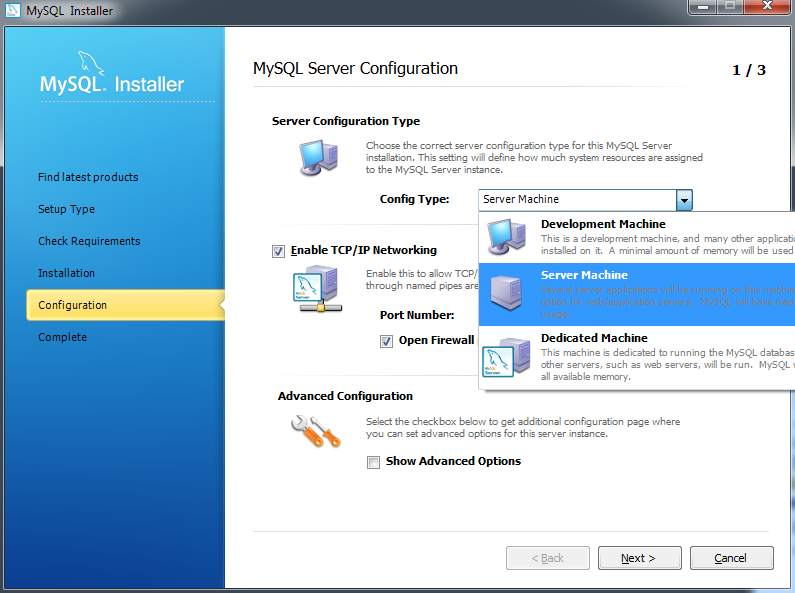
\includegraphics{img/mysql_7.png}
\item
  Now we create uses. Enter a password for the \texttt{root} user.
  \textbf{Please remember the password set here.} Click ``Add User'' to
  create a dedicated user for StarRiver. Use \texttt{sansi} as the
  username and \texttt{starriver} as the password. \textbf{If you
  customize the username or password, make sure you remember what is set
  here as the information will be used later.}
  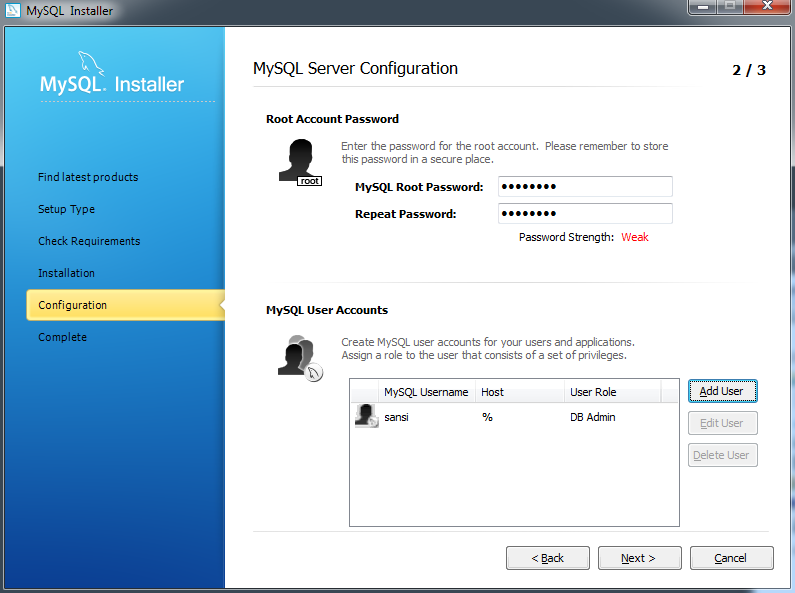
\includegraphics{img/mysql_8.png}
\item
  MySQL Server starts as a Windows service. Just accept the default
  configuration and continue. 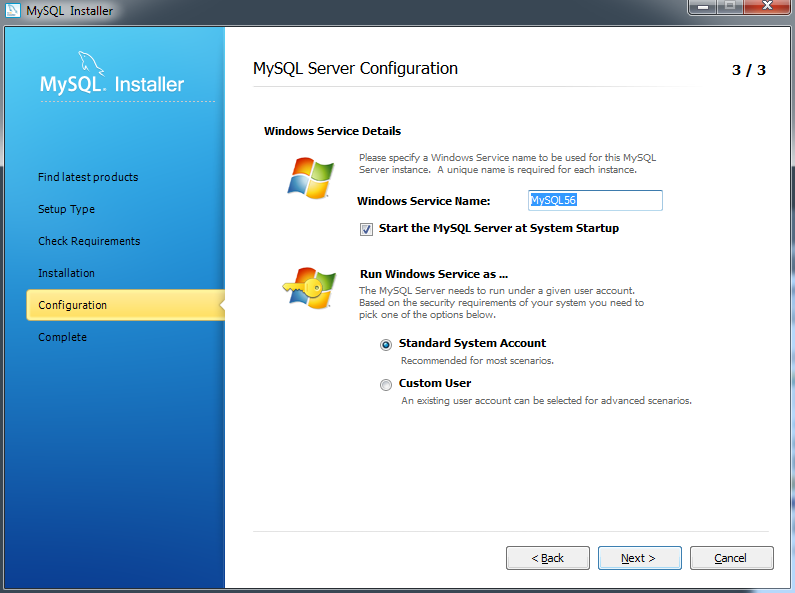
\includegraphics{img/mysql_9.png}
\item
  Continue after the configuration procedure finishes.
  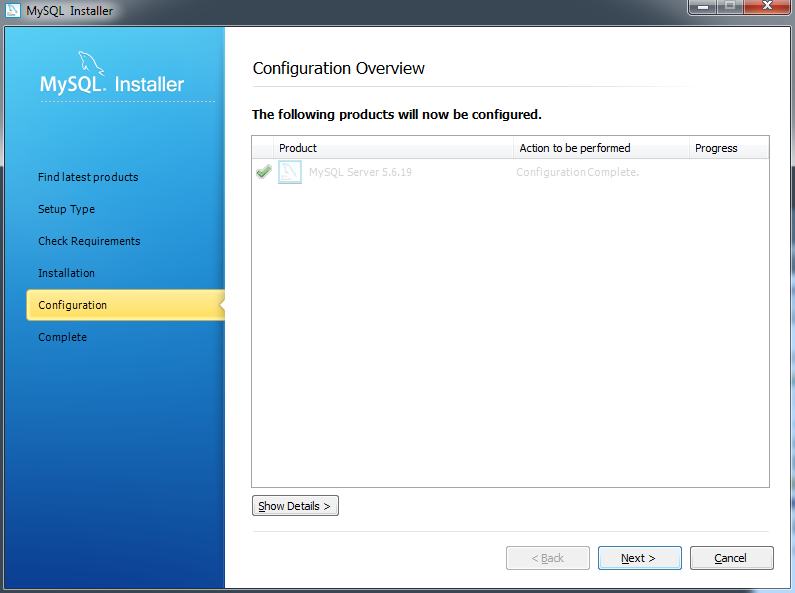
\includegraphics{img/mysql_10.png}
\item
  Installation complete. 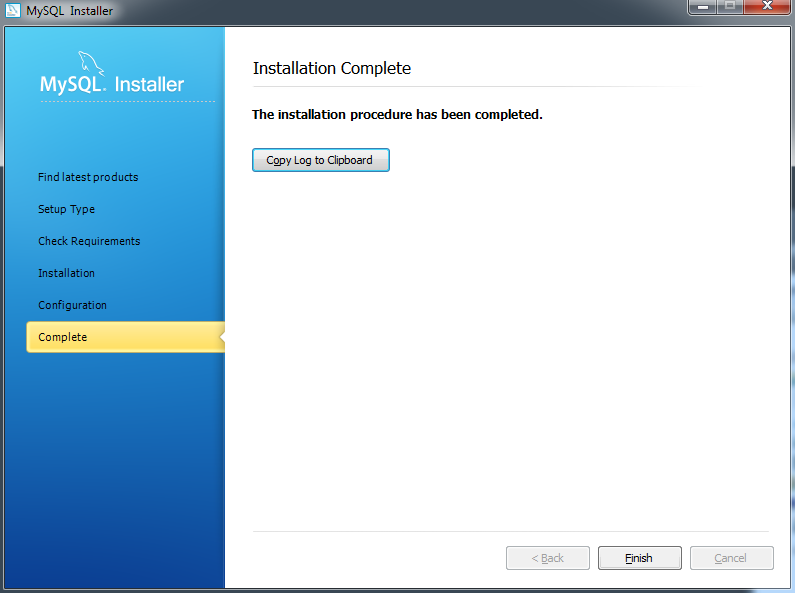
\includegraphics{img/mysql_11.png}
\end{enumerate}

Then install \href{http://dev.mysql.com/downloads/workbench/}{MySQL
Workbench}, a GUI management tool. MySQL Workbench 6.1.7 is adopted in
this example. Accept all defaults during installation.

Finally, create the database structure StarRiver uses.

\begin{enumerate}
\def\labelenumi{\arabic{enumi}.}
\itemsep1pt\parskip0pt\parsep0pt
\item
  Open MySQL Workbench. Click the ``+'' button next to ``MySQL
  Connection'' to create a new MySQL connection.
  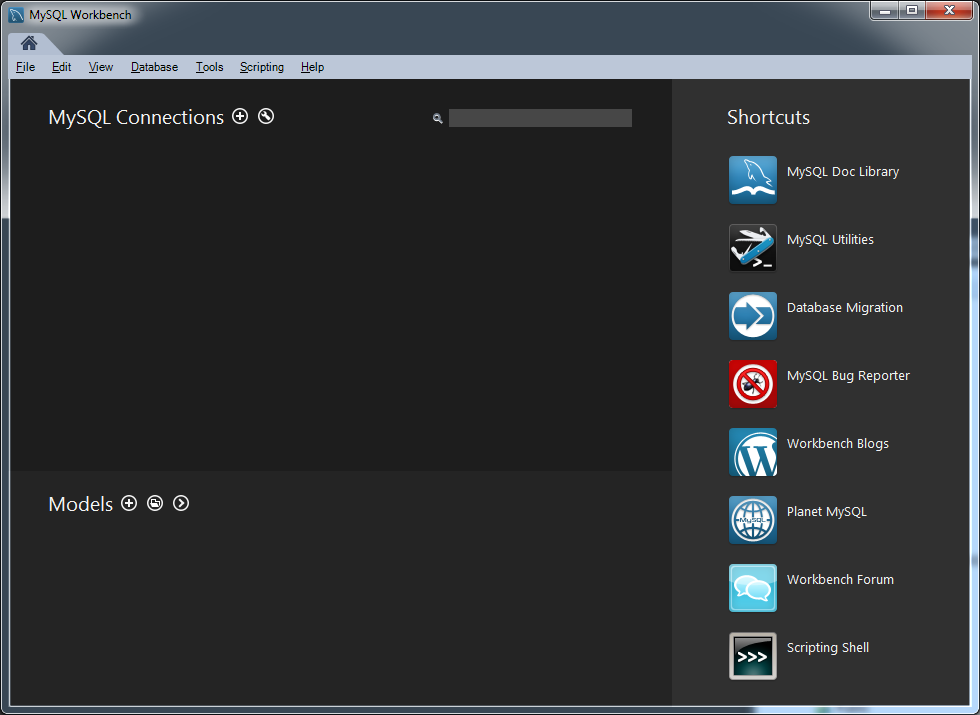
\includegraphics{img/db_init_1.png}
\item
  Enter ``StarRiver'' for connection name, ``sansi'' for username. Click
  ``Store in Vault'' and enter ``starriver'' for password. (If you use a
  custom database user in step 8 during MySQL installation, use that
  instead.) 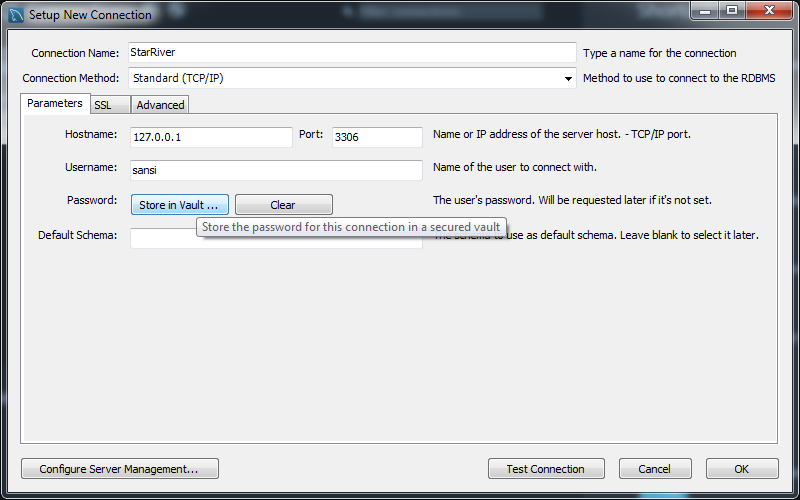
\includegraphics{img/db_init_2.png}
  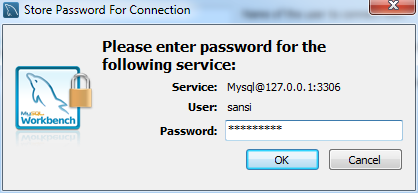
\includegraphics{img/db_init_3.png} Click ``Test Connection''. If
  there is an error, check username and password entered.
  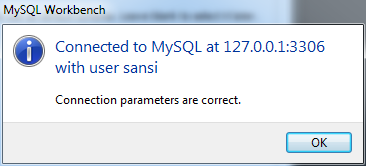
\includegraphics{img/db_init_4.png}
\item
  Click the newly created connection to connect to the database.
  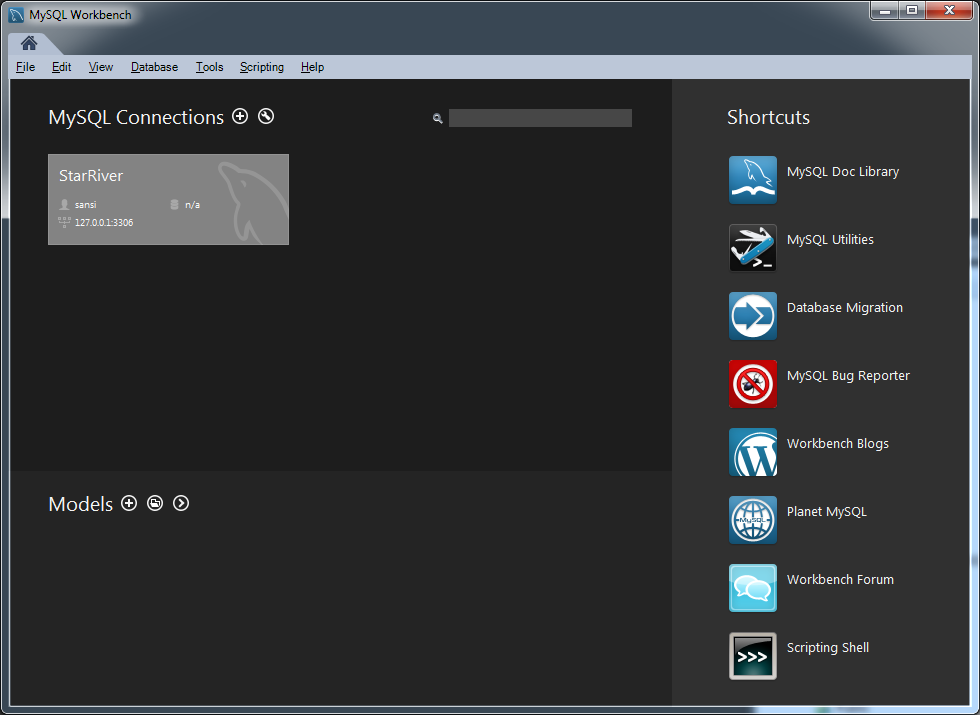
\includegraphics{img/db_init_5.png}
\item
  Select ``File-\textgreater{}Open SQL Script''.
  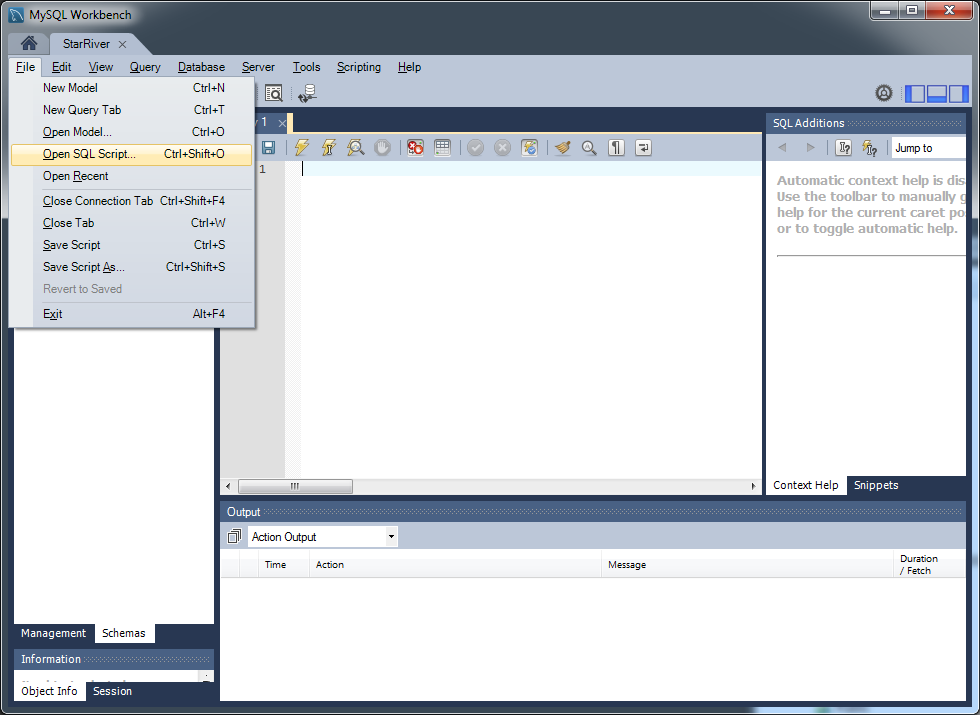
\includegraphics{img/db_init_6.png}
\item
  Open \texttt{init\_db.sql}. Click the execute button highlighted with
  a red box below. 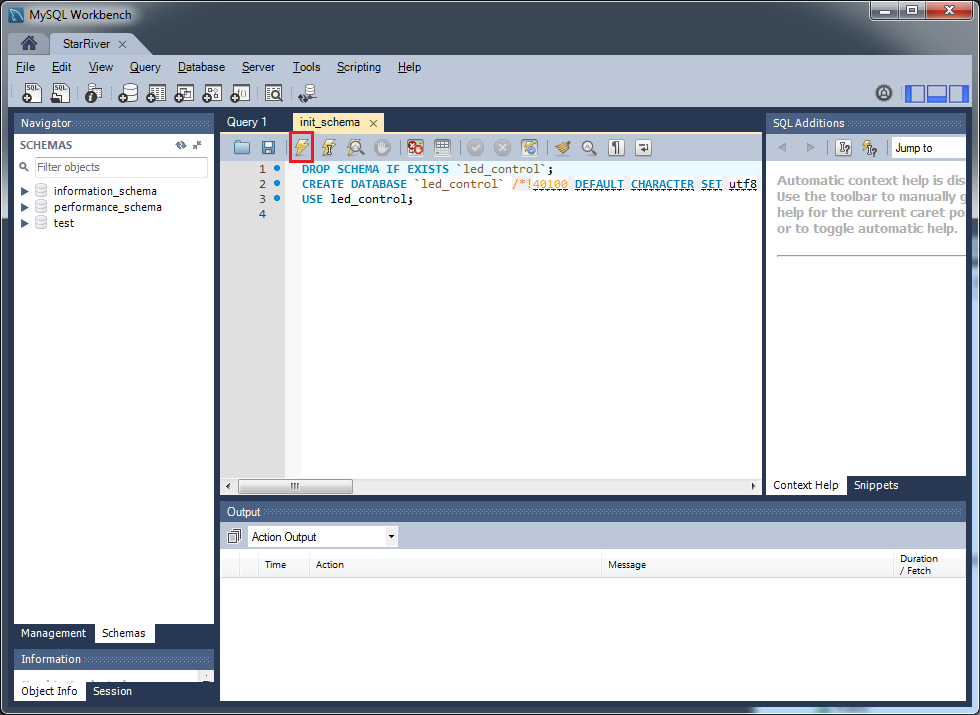
\includegraphics{img/db_init_7.png}
\item
  The script finishes execution with no errors.
  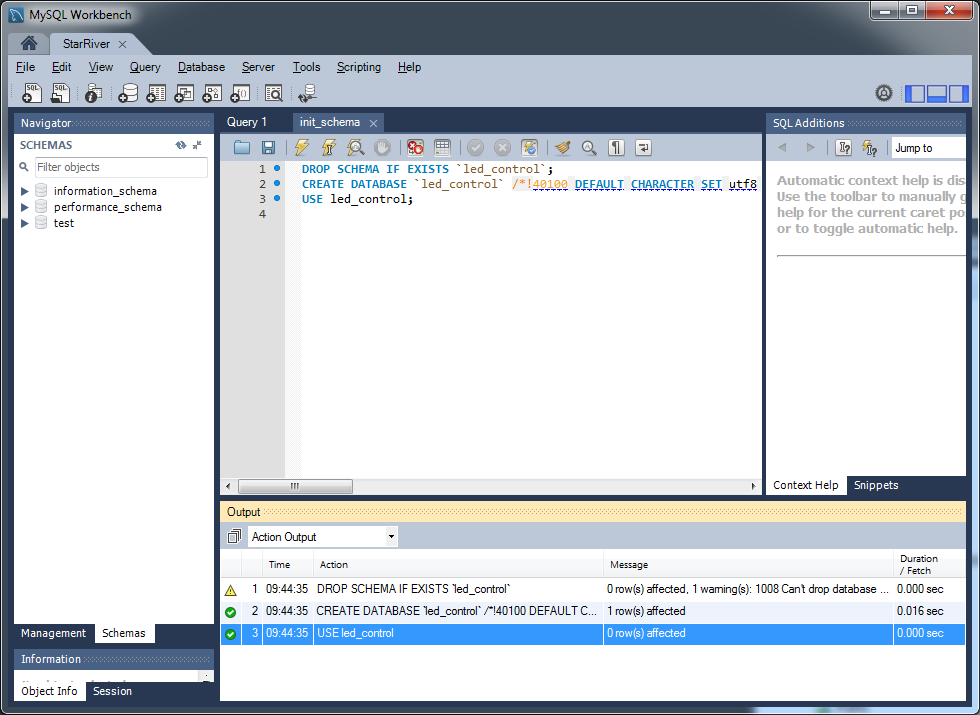
\includegraphics{img/db_init_8.png}
\item
  Execute \texttt{events.sql} the same way.
  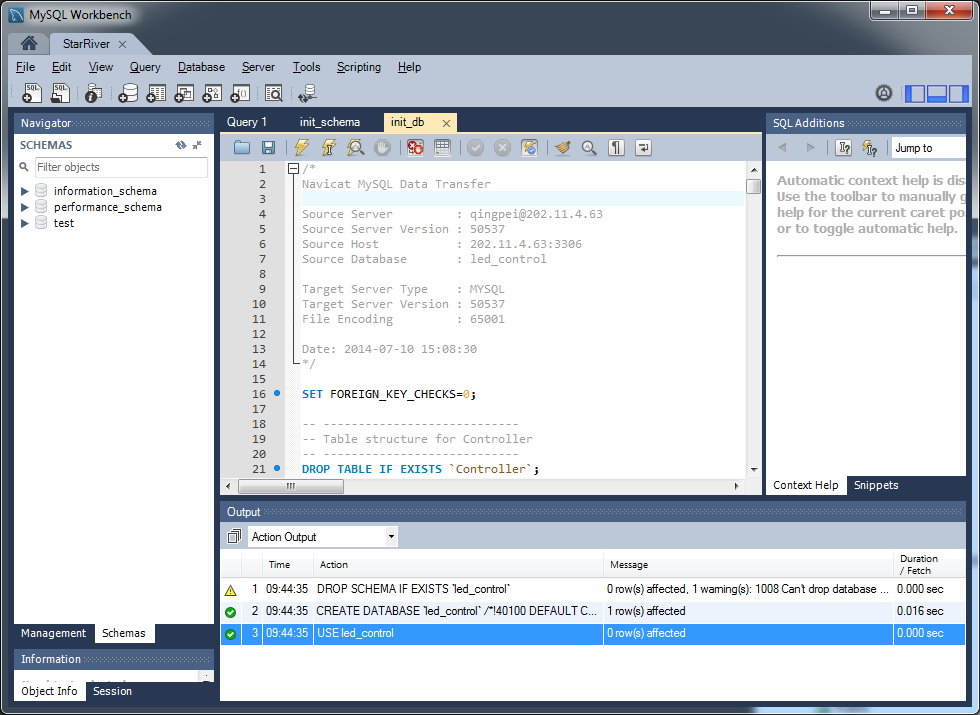
\includegraphics{img/db_init_9.png}
\item
  Check ``Output'' panel for errors.
  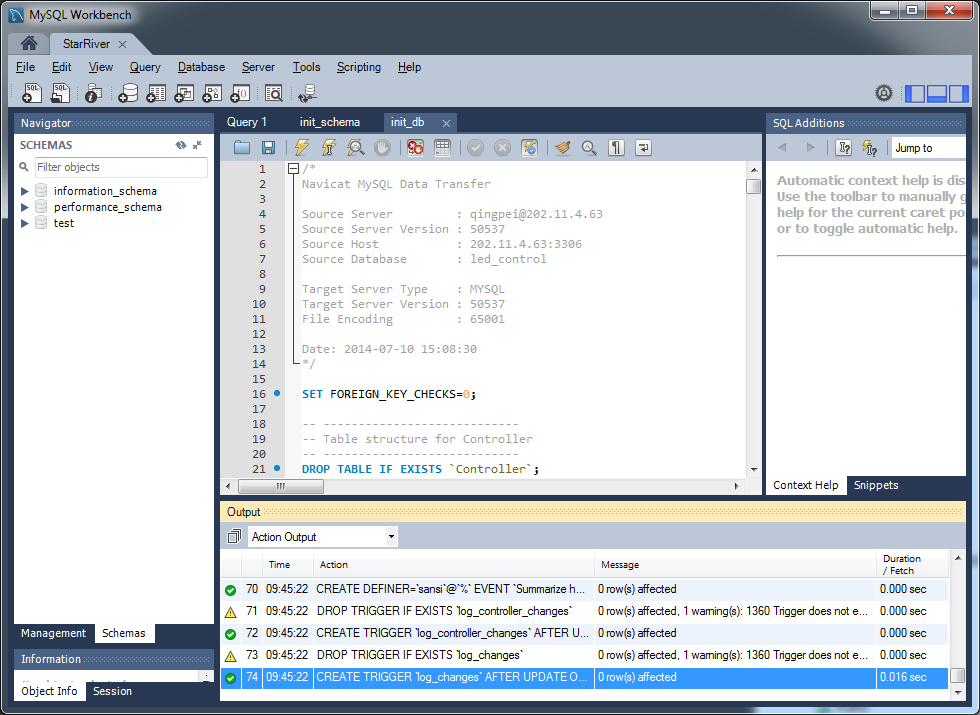
\includegraphics{img/db_init_10.png}
\item
  Click the refresh button in ``Schemas'' panel. Verify the a database
  named \texttt{led\_control} has been setup.
  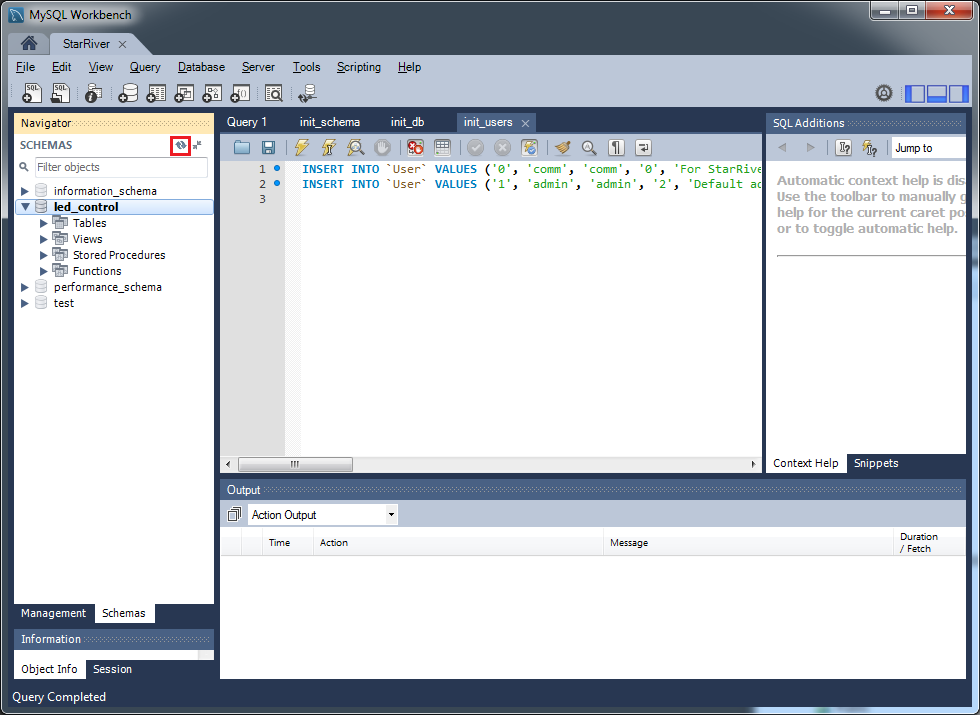
\includegraphics{img/db_init_12.png}
\end{enumerate}

Some extra configuration is necessary for the database server by editing
\texttt{my.ini} in MySQL data path (which is
\texttt{C:\textbackslash{}MySQL\_Data} in this example.)

\begin{figure}[htbp]
\centering
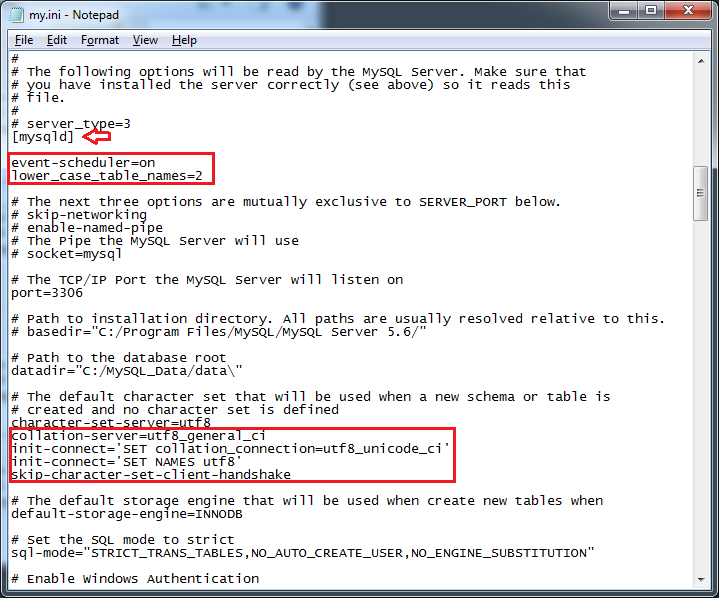
\includegraphics{img/my_ini.png}
\caption{}
\end{figure}

Add the following lines under \texttt{{[}mysqld{]}} section.

\begin{verbatim}
event-scheduler=on
lower_case_table_names=2

collation-server=utf8_general_ci
init-connect='SET collation_connection=utf8_unicode_ci'
init-connect='SET NAMES utf8'
skip-character-set-client-handshake
\end{verbatim}

\textbf{Note that all quote marks are plain
\texttt{\textquotesingle{}}.}

The new configuration will take effect after rebooting the system or
restarting MySQL service.

\subsection{Install StarRiver Communication
Application}\label{install-starriver-communication-application}

Run \texttt{setup.exe} and it just works.

\begin{figure}[htbp]
\centering
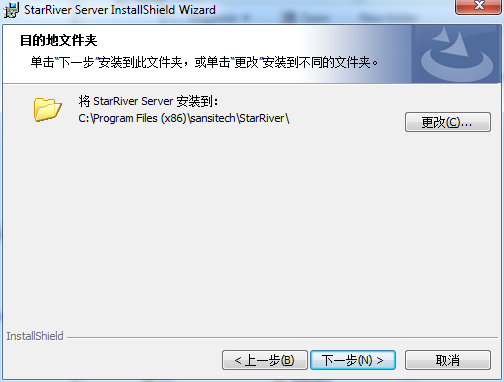
\includegraphics{img/setup.png}
\caption{}
\end{figure}

If you use custom user to connect to the database, you need to edit
\texttt{config.ini} in StarRiver installation path.

\begin{figure}[htbp]
\centering
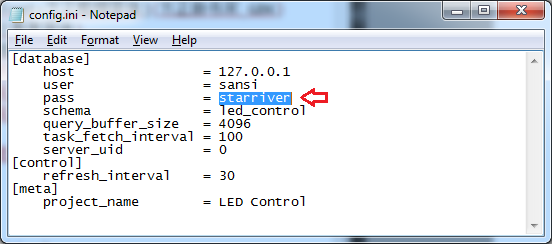
\includegraphics{img/config.png}
\caption{}
\end{figure}

Change the values to allow StarRiver to connect to the database
successfully.
